% Template adapted from the Eurographics SGP 2016 template
\documentclass{6838publ}
\usepackage{6838}
% \input{\string~/.macros}

\SpecialIssuePaper
\electronicVersion 
\ifpdf \usepackage[pdftex]{graphicx} \pdfcompresslevel=9
\else \usepackage[dvips]{graphicx} \fi
\graphicspath{{./assets}}


 
\PrintedOrElectronic

\usepackage{t1enc,dfadobe}
\usepackage{egweblnk}
\usepackage{cite}
\usepackage{lipsum}
\usepackage{amsmath}
\usepackage{amsfonts}
\usepackage{amssymb}

\newcommand\sa{\ensuremath{\mathcal{a}}}
\newcommand\sd{\ensuremath{\mathcal{d}}}
\newcommand\se{\ensuremath{\mathcal{e}}}
\newcommand\sg{\ensuremath{\mathcal{g}}}
\newcommand\sh{\ensuremath{\mathcal{h}}}
\newcommand\si{\ensuremath{\mathcal{i}}}
\newcommand\sj{\ensuremath{\mathcal{j}}}
\newcommand\sk{\ensuremath{\mathcal{k}}}
\newcommand\sm{\ensuremath{\mathcal{m}}}
\newcommand\sn{\ensuremath{\mathcal{n}}}
\newcommand\so{\ensuremath{\mathcal{o}}}
\newcommand\sq{\ensuremath{\mathcal{q}}}
\newcommand\sr{\ensuremath{\mathcal{r}}}
\newcommand\st{\ensuremath{\mathcal{t}}}
\newcommand\su{\ensuremath{\mathcal{u}}}
\newcommand\sv{\ensuremath{\mathcal{v}}}
\newcommand\sw{\ensuremath{\mathcal{w}}}
\newcommand\sx{\ensuremath{\mathcal{x}}}
\newcommand\sy{\ensuremath{\mathcal{y}}}
\newcommand\sz{\ensuremath{\mathcal{z}}}
\newcommand\sA{\ensuremath{\mathcal{A}}}
\newcommand\sB{\ensuremath{\mathcal{B}}}
\newcommand\sC{\ensuremath{\mathcal{C}}}
\newcommand\sD{\ensuremath{\mathcal{D}}}
\newcommand\sE{\ensuremath{\mathcal{E}}}
\newcommand\sF{\ensuremath{\mathcal{F}}}
\newcommand\sG{\ensuremath{\mathcal{G}}}
\newcommand\sH{\ensuremath{\mathcal{H}}}
\newcommand\sI{\ensuremath{\mathcal{I}}}
\newcommand\sJ{\ensuremath{\mathcal{J}}}
\newcommand\sK{\ensuremath{\mathcal{K}}}
\newcommand\sL{\ensuremath{\mathcal{L}}}
\newcommand\sM{\ensuremath{\mathcal{M}}}
\newcommand\sN{\ensuremath{\mathcal{N}}}
\newcommand\sO{\ensuremath{\mathcal{O}}}
\newcommand\sP{\ensuremath{\mathcal{P}}}
\newcommand\sQ{\ensuremath{\mathcal{Q}}}
\newcommand\sR{\ensuremath{\mathcal{R}}}
\newcommand\sS{\ensuremath{\mathcal{S}}}
\newcommand\sT{\ensuremath{\mathcal{T}}}
\newcommand\sU{\ensuremath{\mathcal{U}}}
\newcommand\sV{\ensuremath{\mathcal{V}}}
\newcommand\sW{\ensuremath{\mathcal{W}}}
\newcommand\sX{\ensuremath{\mathcal{X}}}
\newcommand\sY{\ensuremath{\mathcal{Y}}}
\newcommand\sZ{\ensuremath{\mathcal{Z}}}

\newcommand\ba{\ensuremath{\mathbf{a}}}
\newcommand\bb{\ensuremath{\mathbf{b}}}
\newcommand\bc{\ensuremath{\mathbf{c}}}
\newcommand\bd{\ensuremath{\mathbf{d}}}
\newcommand\be{\ensuremath{\mathbf{e}}}
\newcommand\bg{\ensuremath{\mathbf{g}}}
\newcommand\bh{\ensuremath{\mathbf{h}}}
\newcommand\bi{\ensuremath{\mathbf{i}}}
\newcommand\bj{\ensuremath{\mathbf{j}}}
\newcommand\bk{\ensuremath{\mathbf{k}}}
\newcommand\bl{\ensuremath{\mathbf{l}}}
\newcommand\bn{\ensuremath{\mathbf{n}}}
\newcommand\bo{\ensuremath{\mathbf{o}}}
\newcommand\bp{\ensuremath{\mathbf{p}}}
\newcommand\bq{\ensuremath{\mathbf{q}}}
\newcommand\br{\ensuremath{\mathbf{r}}}
\newcommand\bs{\ensuremath{\mathbf{s}}}
\newcommand\bt{\ensuremath{\mathbf{t}}}
\newcommand\bu{\ensuremath{\mathbf{u}}}
\newcommand\bv{\ensuremath{\mathbf{v}}}
\newcommand\bw{\ensuremath{\mathbf{w}}}
\newcommand\bx{\ensuremath{\mathbf{x}}}
\newcommand\by{\ensuremath{\mathbf{y}}}
\newcommand\bz{\ensuremath{\mathbf{z}}}
\newcommand\bA{\ensuremath{\mathbf{A}}}
\newcommand\bB{\ensuremath{\mathbf{B}}}
\newcommand\bC{\ensuremath{\mathbf{C}}}
\newcommand\bD{\ensuremath{\mathbf{D}}}
\newcommand\bE{\ensuremath{\mathbf{E}}}
\newcommand\bF{\ensuremath{\mathbf{F}}}
\newcommand\bG{\ensuremath{\mathbf{G}}}
\newcommand\bH{\ensuremath{\mathbf{H}}}
\newcommand\bI{\ensuremath{\mathbf{I}}}
\newcommand\bJ{\ensuremath{\mathbf{J}}}
\newcommand\bK{\ensuremath{\mathbf{K}}}
\newcommand\bL{\ensuremath{\mathbf{L}}}
\newcommand\bM{\ensuremath{\mathbf{M}}}
\newcommand\bN{\ensuremath{\mathbf{N}}}
\newcommand\bO{\ensuremath{\mathbf{O}}}
\newcommand\bP{\ensuremath{\mathbf{P}}}
\newcommand\bQ{\ensuremath{\mathbf{Q}}}
\newcommand\bR{\ensuremath{\mathbf{R}}}
\newcommand\bS{\ensuremath{\mathbf{S}}}
\newcommand\bT{\ensuremath{\mathbf{T}}}
\newcommand\bU{\ensuremath{\mathbf{U}}}
\newcommand\bV{\ensuremath{\mathbf{V}}}
\newcommand\bW{\ensuremath{\mathbf{W}}}
\newcommand\bX{\ensuremath{\mathbf{X}}}
\newcommand\bY{\ensuremath{\mathbf{Y}}}
\newcommand\bZ{\ensuremath{\mathbf{Z}}}
\newcommand\Ba{\ensuremath{\mathbb{a}}}
\newcommand\Bb{\ensuremath{\mathbb{b}}}
\newcommand\Bc{\ensuremath{\mathbb{c}}}
\newcommand\Bd{\ensuremath{\mathbb{d}}}
\newcommand\Be{\ensuremath{\mathbb{e}}}
\newcommand\Bf{\ensuremath{\mathbb{f}}}
\newcommand\Bg{\ensuremath{\mathbb{g}}}
\newcommand\Bh{\ensuremath{\mathbb{h}}}
\newcommand\Bi{\ensuremath{\mathbb{i}}}
\newcommand\Bj{\ensuremath{\mathbb{j}}}
\newcommand\Bk{\ensuremath{\mathbb{k}}}
\newcommand\Bl{\ensuremath{\mathbb{l}}}
\newcommand\Bm{\ensuremath{\mathbb{m}}}
\newcommand\Bn{\ensuremath{\mathbb{n}}}
\newcommand\Bo{\ensuremath{\mathbb{o}}}
\newcommand\Bp{\ensuremath{\mathbb{p}}}
\newcommand\Bq{\ensuremath{\mathbb{q}}}
\newcommand\Br{\ensuremath{\mathbb{r}}}
\newcommand\Bs{\ensuremath{\mathbb{s}}}
\newcommand\Bt{\ensuremath{\mathbb{t}}}
\newcommand\Bu{\ensuremath{\mathbb{u}}}
\newcommand\Bv{\ensuremath{\mathbb{v}}}
\newcommand\Bw{\ensuremath{\mathbb{w}}}
\newcommand\Bx{\ensuremath{\mathbb{x}}}
\newcommand\By{\ensuremath{\mathbb{y}}}
\newcommand\Bz{\ensuremath{\mathbb{z}}}
\newcommand\BA{\ensuremath{\mathbb{A}}}
\newcommand\BB{\ensuremath{\mathbb{B}}}
\newcommand\BC{\ensuremath{\mathbb{C}}}
\newcommand\BD{\ensuremath{\mathbb{D}}}
\newcommand\BE{\ensuremath{\mathbb{E}}}
\newcommand\BF{\ensuremath{\mathbb{F}}}
\newcommand\BG{\ensuremath{\mathbb{G}}}
\newcommand\BH{\ensuremath{\mathbb{H}}}
\newcommand\BI{\ensuremath{\mathbb{I}}}
\newcommand\BJ{\ensuremath{\mathbb{J}}}
\newcommand\BK{\ensuremath{\mathbb{K}}}
\newcommand\BL{\ensuremath{\mathbb{L}}}
\newcommand\BM{\ensuremath{\mathbb{M}}}
\newcommand\BN{\ensuremath{\mathbb{N}}}
\newcommand\BO{\ensuremath{\mathbb{O}}}
\newcommand\BP{\ensuremath{\mathbb{P}}}
\newcommand\BQ{\ensuremath{\mathbb{Q}}}
\newcommand\BR{\ensuremath{\mathbb{R}}}
\newcommand\BS{\ensuremath{\mathbb{S}}}
\newcommand\BT{\ensuremath{\mathbb{T}}}
\newcommand\BU{\ensuremath{\mathbb{U}}}
\newcommand\BV{\ensuremath{\mathbb{V}}}
\newcommand\BW{\ensuremath{\mathbb{W}}}
\newcommand\BX{\ensuremath{\mathbb{X}}}
\newcommand\BY{\ensuremath{\mathbb{Y}}}
\newcommand\BZ{\ensuremath{\mathbb{Z}}}
\newcommand\balpha{\ensuremath{\mbox{\boldmath$\alpha$}}}
\newcommand\bbeta{\ensuremath{\mbox{\boldmath$\beta$}}}
\newcommand\btheta{\ensuremath{\mbox{\boldmath$\theta$}}}
\newcommand\bphi{\ensuremath{\mbox{\boldmath$\phi$}}}
\newcommand\bpi{\ensuremath{\mbox{\boldmath$\pi$}}}
\newcommand\bpsi{\ensuremath{\mbox{\boldmath$\psi$}}}
\newcommand\bmu{\ensuremath{\mbox{\boldmath$\mu$}}}

\newcommand\R{\ensuremath{\mathbb{R}}} % Real numbers
\newcommand\Z{\ensuremath{\mathbb{Z}}} % Integers


\newcommand{\norm}[1]{\left\lVert#1\right\rVert}
\newcommand\inner[2]{\ensuremath{\left< #1, #2 \right>}} % Inner product
\DeclareMathOperator*{\diag}{diag} % Diagonal matrix
\newcommand\p[1]{\ensuremath{\left( #1 \right)}} % Parenthesis ()
\newcommand\pa[1]{\ensuremath{\left\langle #1 \right\rangle}} % <>
\newcommand\pb[1]{\ensuremath{\left[ #1 \right]}} % []
\newcommand\pc[1]{\ensuremath{\left\{ #1 \right\}}} % {}


\title[]{Optimal Transport based Probabilistic Diffeomorphic Registration}

\author[P.W.]
       {Peiqi Wang
        \\
        MIT Department of Electrical Engineering and Computer Science\\
       }

\begin{document}

\teaser{
 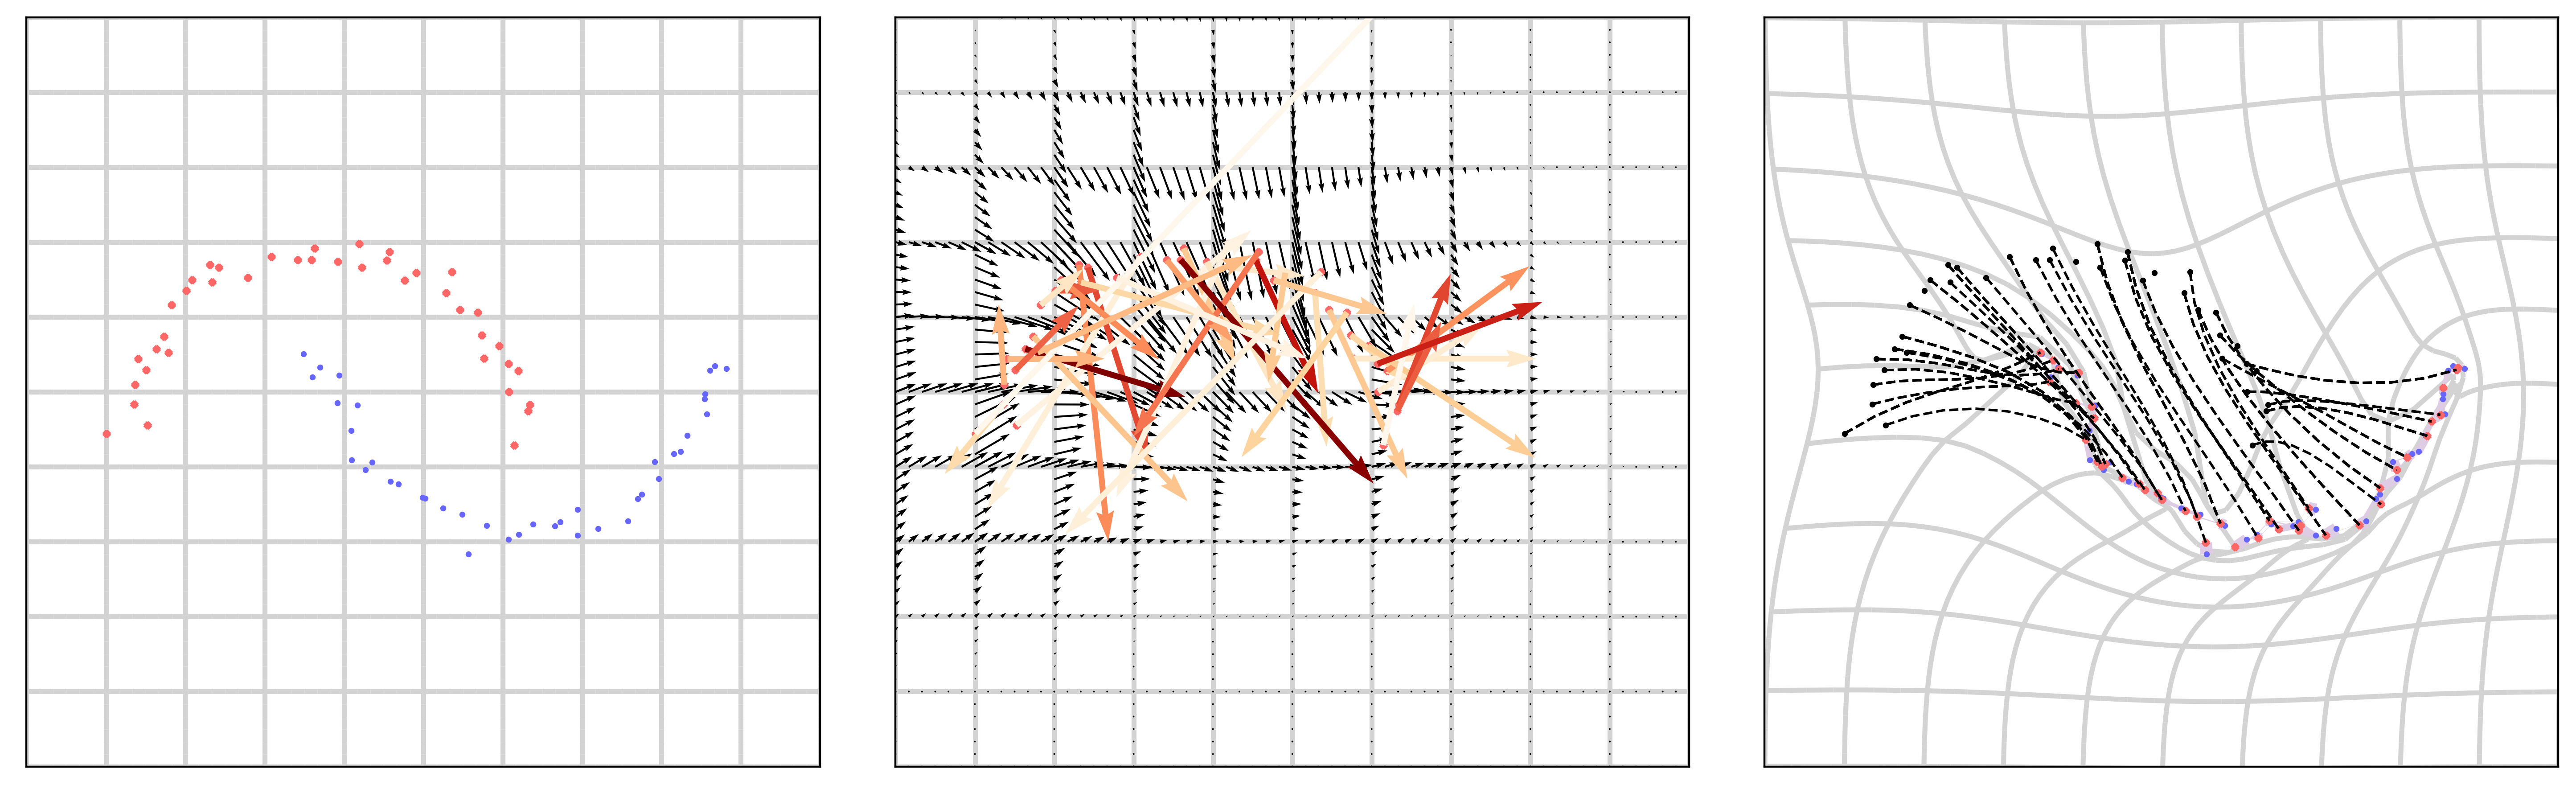
\includegraphics[width=.9\linewidth]{{assets/amoeba/plt_lddmm_points}}
 \centering
  \caption{The red amoeba is registered to blue amoeba. A valid diffeomorphic transformation can be generated from per-particle momenta (orange arrow) by solving a set of Geodesic equations (black dashed line). On the right, we can visualize variance of the effect of random transformation on shape as a heatmap. Although the two shapes is matched almost perfectly, the two legs flips over itself respectively and we are able to spot this mistake from the uncertainty heatmap.}
\label{fig:teaser}
}

\maketitle

\begin{abstract}

\end{abstract}

\section{Introduction}

 
% narrow in no topic: remind this is a graphics paper, need to help them to figure out what topic and area of research. no need to wax poetic about topic's importance


% dig a hole: convince reader there is a problem with the state of the world. prior work may exist but its missing something important or there is a missing opportunity. the reading should be drooling for a bright future just out of reach

Diffeomorphic registration of shapes with unknown correspondence is an important step in medical data processing. The choice of similarity metric for good matching distinguishes the different algorithms in this domain. Recent work explored the use of entropic regularized wasserstein distance as a global measure of similarity between encoding of shapes as discrete measures \cite{feydyOptimalTransportDiffeomorphic2017a,feydyFastScalableOptimal2019}. However, a point estimate of the transformation yield errors that may invalidate downstream processing pipelines or misguide clinical decision making. Additionally, solution is sensitive to hyperparameters of the problem, requiring manual tuning for each new shape. 

% fill the hole: to show reader how/why the paper will fix these problems and deliver us into a better place. don't need a whirlwind summary of technical details, but need reader's convinced to keep reading. 

We propose to extend optimal transport based diffeomorphic registration to probabilistic setting. Our method interprets the diffeomorphic transformation as a random variable, and estimates its parameters using variational inference. In particular, we find diffeomorphic maps that minimize the average Wasserstein distance between shapes. Naturally, the probabilistic formulation provides us with uncertainty estimates of both the transformation as well as the uncertainty of its effect on shapes. Hyperparameters such as the degree of smoothness of the transformation parameterizes the variational distribution, and thus can be optimized. However, the inference procedure requires repeated sampling of valid diffeomorphic transformations to approximate the average cost. To alleviate the computational burden, we explored links to sparse Gaussian Process, specifically interdomain inducing variables, as a way to alleviate this concern \cite{figueiras-vidalInterdomainGaussianProcesses2009a}.


\section{Related Work}

\subsection{Diffeomorphic Registration}

The large deformation registration of landmarks (point sets) and images as a variational problem that solves for a smooth time-varying velocity field that matches the two objects according to some measure of similarity \cite{joshiLandmarkMatchingLarge2000,begComputingLargeDeformation2005}. \cite{millerGeodesicShootingComputational2006,vialardDiffeomorphic3DImage2012} makes connection to optimal control, and showed that large deformation diffeormorphisms obeys conservation of momentum, and that points/images evolve according to a set of Geodesic Equations completely determined by its initial momentum. This observation prompted the development of \textit{geodesic shooting} methods that optimizes for initial momentum for point sets and meshes \cite{vaillantStatisticsDiffeomorphismsTangent2004,allassonniereGeodesicShootingDiffeomorphic2005} and later extended to images \cite{vialardDiffeomorphic3DImage2012}. We relie on geodesic shooting methods in our formulation.


\subsection{Registration Uncertainty}






% Descriptions of and citations to academic research papers and/or existing software products related to your work.  Here is an example of how to cite a paper~\cite{solomon-2016}; see \texttt{6838bibsample.bib} for bibliography entries.


\section{Technical Approach}\label{sec:technical_approach}


\subsection{Diffeomorphic Registration}
% We follow the usual setup for registering unlabeled point sets using geodesic shooting \cite{vaillantStatisticsDiffeomorphismsTangent2004}. 


Let $\Omega \subset\R^D$ be a low dimensional ambient space. Let $x := (x^1,\cdots,x^n)\subset \R^{N\times D}$, $y := (y^1,\cdots,y^n)\subset\Omega^{N\times D}$ be source and target points respectively. The goal of diffeomorphic registration of point sets is to transform $x$ via a diffeomorphic mapping $\varphi$ s.t. $\varphi(x)$ is close to $y$ according to some similarity metric $\sL(\varphi(x),y)$.


Let the space of smooth velocity fields $V$ as a rkhs over $\Omega$ characterized by kernel $\overline{k}:\Omega\times\Omega\to\R^{D\times D}$ satisfying vector-valued reproducing property $\inner{\overline{k}(x,\cdot)y}{v}_{V} = \inner{v(x)}{y}_{\R^D}$ for all $y\in\R^D, v\in V$. For our purposes, we consider an equivalent scalar-valued rkhs with kernel $k:\Omega\times[D]\times\Omega\times[D] \to\R$ where $\overline{k}(x,x')_{dd'} = k((x,d),(x',d'))$. A diffeomorphism can be constructed via flows , i.e. solutions to an ODE problem $\varphi_t$, $\dot{\varphi}_t = v_t\circ \varphi_t, \varphi_0 = \text{Id}$, of a sufficiently smooth velocity field, i.e. $\int_0^1 \norm{v_t}_V\, dt<\infty$. The large deformation registration problem solves for a time-varying velocity field $v_t\in V$ matching $x$ to $y$.
\begin{align}
    \min_{v_t:t\in [0,1]} \,
        &\frac{1}{2} \int_0^1 \norm{v_t}_V^2 \, dt + \sL(\varphi(x),y)
\end{align}

\subsection{Geodesic Shooting}

Let $q_t^i = \varphi_t(x^i) \in \R^D$ be application of transformation $\varphi_t$ to point $x^i$. Denote $q_t = (q_t^1, \cdots, q_t^N) \in \R^{ND}$ as action of $\varphi_t$ to a set of points and $K(q_t,q_t) \in \R^{ND\times ND}$ be kernel matrix for vectorized velocity vector field at $q_t$. \cite{joshiLandmarkMatchingLarge2000} argues for a Lagrangian view of previous Eulerian problem - it suffices to solve for the flow velocity $\dot{q}_t$ of particles,
\begin{align}
    \min_{\dot{q}_t:t\in [0,1]}
        &\frac{1}{2} \int_0^1 \inner{\dot{q}_t}{K(q_t,q_t)^{-1}\dot{q}_t} \, dt + \sL(\varphi(x),y)
\end{align}
and that the resulting flow velocity in the Eulerian coordinates $\Omega$ can be interpolated from $\dot{q}_t$,
\begin{align}
    v_t(x)
        = K(x, q_t) p_t
    \quad\quad
    p_t
        = K(q_t, q_t)^{-1} \dot{q}_t
\end{align}
where $p_t^i \in \R^{D}$ is the momenta associated with point $q_t^i$. As a side note, this interpolation is akin to computing posterior mean of a gaussian process regression of velocity fields, i.e. $v_t(x) = K(x,q_t) K(q_t,q_t)^{-1} \dot{q}_t$. Note the integrand of rkhs norm can be viewed as Lagrangian of of a system of ND particles. \cite{millerGeodesicShootingComputational2006} argues the dynamics of these particles in canonical coordinates $(q_t,p_t)$ follows the Geodesic equations
\begin{align}
    \dot{q}_t
        = \frac{\partial \sH(q_t,p_t)}{\partial p}
    \quad\quad
    \dot{p}_t
        = - \frac{\partial \sH(q_t,p_t)}{\partial q}
    \label{eq:geodesic_equations}
\end{align}
with initial condition $q_0 = x, p_0$, and that the Hamiltonian 
\begin{align}
    \sH(q_t,p_t) = \frac{1}{2}\inner{p_t}{K(q_t,q_t)p_t} = \frac{1}{2}\inner{K(q_t,q_t)^{-1}\dot{q}_t}{\dot{q}_t}  
\end{align}
is preseved by the flow, $\sH(q_0,p_0)  = \sH(q_t,p_t)$ for all $t\in [0,1]$ (see Figure~(\ref{fig:plt_shooting})). Therefore, $\int_0^1 \sH(q_t,p_t) \, dt = \sH(q_0, p_0) = \frac{1}{2} \inner{ p_0 }{ K(q_0,q_0) p_0 }$. We arrive at a registration problem where we optimize over the initial \textit{shooting momentum} $p_0$,
\begin{align}
    \min_{p_0\in\R^{ND}} \,
        \frac{1}{2} \inner{ p_0 }{ K(x,x) p_0 } + \sL(\varphi(x),y)
    \label{eq:optimization_momentum_landmark}
\end{align}
where $\varphi = q_1 \in \R^{ND}$. Optimization involves a forward integration of $(q_t,p_t)$ via (\ref{eq:geodesic_equations}) to get transformed particles $q_1$, compute the gradient of objective (\ref{eq:optimization_momentum_landmark}) with respect to initial momentum, and do gradient update iteratively. 


\begin{center} 
\begin{figure}[t]
    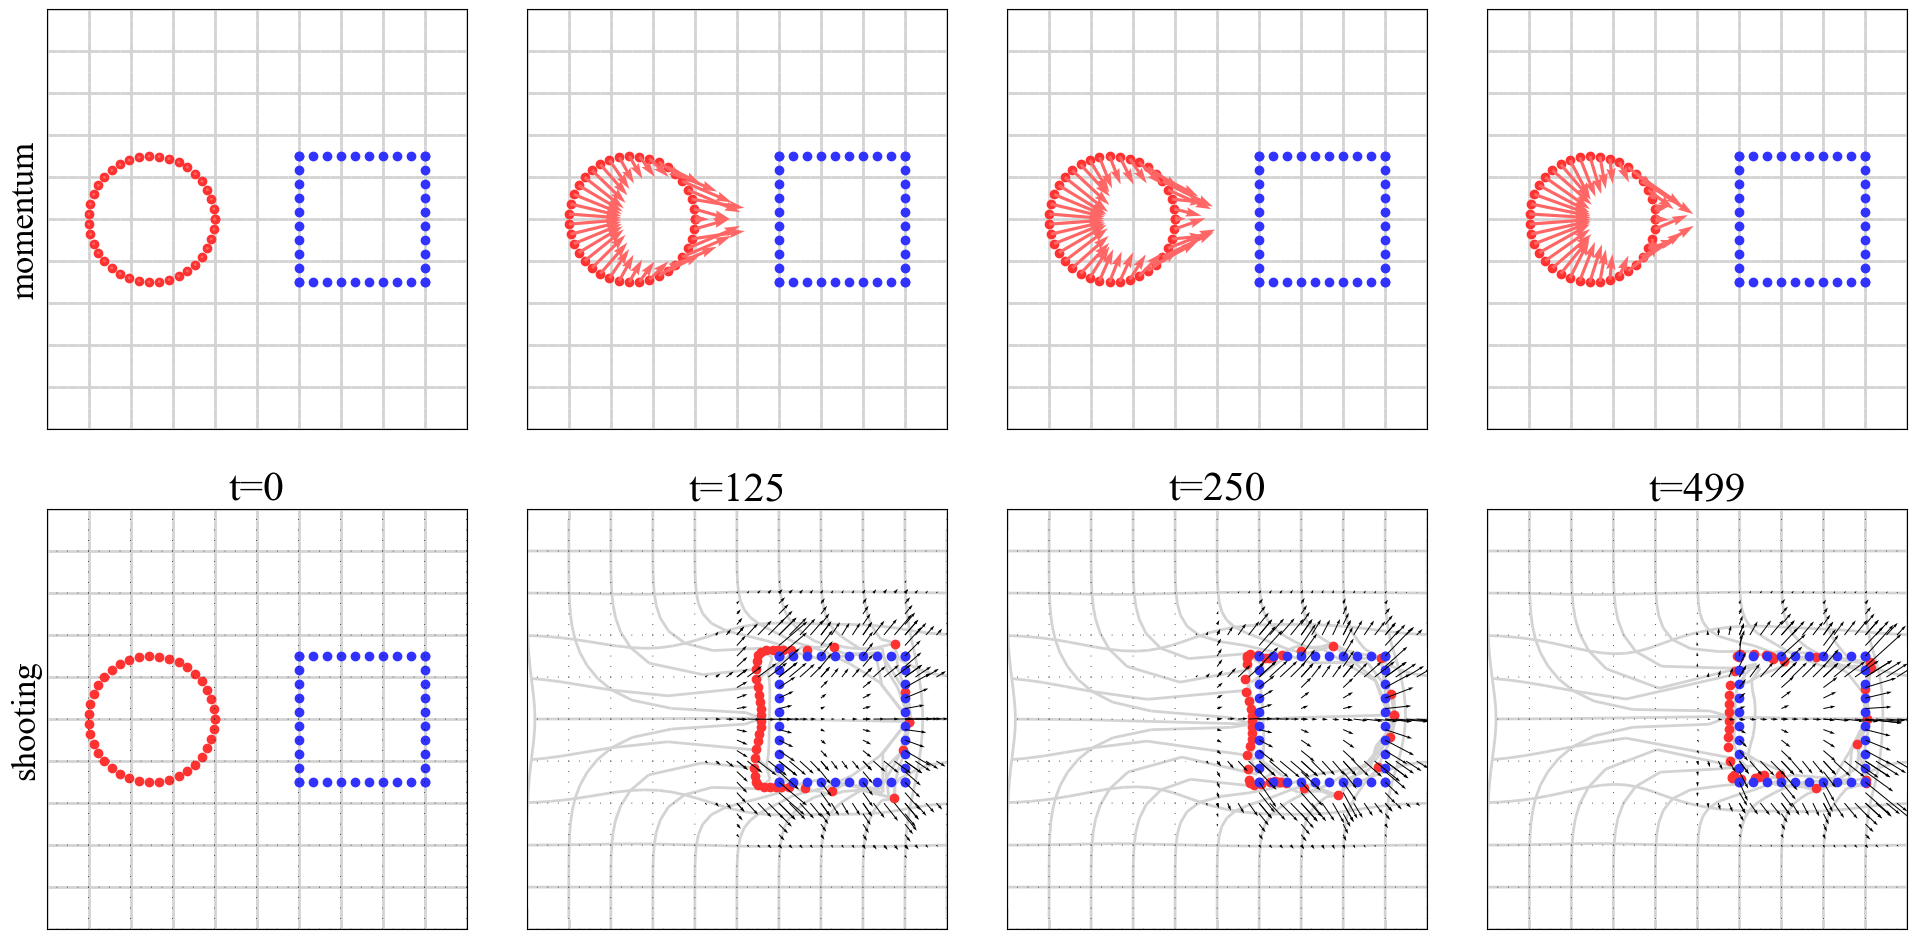
\includegraphics[width=\linewidth]{assets/plt_shooting} 
    \caption{Geodesic shooting with an Euler integrator with time step of $\delta t = .1$. The velocity field is represented using a radial basis kernel with $\sigma=.25$. We show trajectory of $q_t$ (red dots) with momentum $p_t$ (blue arrow) and interpolated velocity fields at grid points (black). We see Hamiltonian is approximately conserved!}
    \label{fig:plt_shooting}
\end{figure} 
\end{center} 



\subsection{Monge's and Kantorovich's formulation}

Given $a,b \in \triangle^{n-1}$, where $\triangle^{n-1}$ is unit simplex. $\alpha = \sum_{i=1}^n a_i \delta_{x_i}, \beta = \sum_{j=1}^m b_j \delta_{y_i}$ are discrete measures. The optimal transport problem tries to find a map that associate each point $x_i$ to a single point $y_j$ such that masses are preserved. This corresponds to classical Monge's formulation of optimal transport
\begin{align}
    \min_{T:\sX\to\sY: T_{\#}\alpha = \beta}\,
        &\sum_{i=1}^n c(x_i, T(x_i))
\end{align}



where $c:\sX\times\sY \to\R$ is cost defined over support of measures, and that the constraints is simply that $T$ is constrained to be a pushforward from $\alpha$ to $\beta$. The problem with Monge's formulation is that the problem is combinatorial and nonconvex, so hard to solve. Kantorovich relax the deterministic nature of transport map, allowing mass at each source point split and be dispatched to multiple target points. This information is encoded in $P\in\R^{n\times m}_+$, where $P_{ij}$ describes amount of mass flowing from $x_i$ to $y_j$. The Kantorovich formulation of optimal transport for discrete measures is then
\begin{align}
    \min_{P\in\R^{n\times m}_+: P1_m = a,\, P^T1_n = b}\,
        &\inner{C}{P}
\end{align}
where the constraints specifies the set of admissible transport map to be a coupling of marginals $\alpha,\beta$ and $C\in\R^{n\times m}$ is the cost matrix, i.e. $C_{ij} = c(x_i,y_j)$. The optimization problem is a linear program and hence can be easily solved using simplex algorithm. In addition, we can instead solve the dual problem, and because of zero duality gap, equivalently solves the primal problem,
\begin{align}
    \max_{f,g\in\R^n\times\R^m: f_i+g_j \leq C_{ij}}\,
        &\inner{f}{a} + \inner{g}{b} 
\end{align}
where $f,g$ are called dual potential.

\section{Entropic Regularization}

Regularizing the original optimal transport problem brings computational and statistical benefits. In particular, the optimization problem can now be solved with fast matrix scaling algorithms that scales with strength of regularization. In addition, the sample efficiency for regularized problem is also superior. The entropy and KL divergence of coupling between two discrete measure is given by
\begin{align}
    H(P)
        &= -\sum_{i,j} P_{ij}(\log(P_{ij})-1)
        = - \inner{P}{\log P} + 1^TP1 \\
    \text{KL}(P\Vert K)
        &= \sum_{i,j} P_{ij} \log \frac{P_{ij}}{K_{ij}} - P_{ij} + K_{ij}
        = \inner{P}{\log(P\oslash K)} + 1^T(K-P)1
\end{align}
where taking logarithm and subtraction are elementwise operations. The entropic regularized problem
\begin{align}
    \min_{P\in\R^{n\times m}_+:P1_m=a,P^T1_n=b}\,
        &\inner{P}{C} - \epsilon H(P)
    \label{eq:opt_entropic_regularized_ot}
\end{align}
We can interpret primal objective as the information projection of the Gibbs kernel $K\in\R^{n\times m}$ where $K_{ij}=e^{-\frac{C_{ij}}{\epsilon}}$ onto the admissible couplings $U(a,b)=\pc{P\in\R^{n\times m}_+\mid P1_m=a,\, P^T1_n=b}$.
\begin{align}
    \inner{P}{C} + \epsilon\inner{P}{\log P} - \epsilon 1^T P 1
        = \epsilon \inner{P}{\log\left(P \oslash e^{-C/\epsilon} \right)} - \epsilon 1^TP1 + \epsilon 1^Te^{-C/\epsilon}1
        = \epsilon \text{KL}(P\Vert K)
\end{align}

\subsection{Sinkhorn's Algorithm}

We can solve regularized optimal transport problem with Sinkhorn algorithm \cite{cuturiSinkhornDistancesLightspeed2013}. The basic idea is to write the 1st order optimality condition for the primal variables for the Lagrangian,
\begin{align}
    \sL(P,f,g)
        &= \inner{P}{C} - \epsilon H(P) - \inner{f}{P1_m-a}- \inner{g}{P^T1_n-b} \\
    \partial \sL(P,f,g)/\partial P_{ij}
        &= C_{ij} + \epsilon \log(P_{ij}) - f_i - g_j = 0
        \quad\Rightarrow\quad
        P_{ij} = e^{(-C_{ij}+f_i+g_j)/\epsilon}
\end{align}

% Note optimal $P$ can be written as scaling of Gibbs kernel row-wise by $u=e^{f/\epsilon}$ and column-wise by $v=e^{g/\epsilon}$, i.e. $P=\diag(u)K \diag(v)$. Substitute expression for $P$ into marginal constraints, get $a = \diag(u) K \diag(v) 1_m = u\odot (Kv)$ and $b = v\odot (K^T u)$. The Sinkhorn's algorithm updates $u,v$ alternatingly
\begin{align}
    u^{(\ell+1)} 
        \leftarrow a \oslash (Kv^{(\ell)}) 
    \quad\quad
    v^{(\ell+1)}
        \leftarrow b \oslash (K^Tu^{(\ell+1)})
\end{align}
Each iteration of the algorithm uses $\sO(nm)$ computation for matrix-vector products and can be accelerated to $\sO(n\log n)$ using convolution if suppport is over gridded space. 
\subsection{Log-domain Stabilization}

Sinkhorn's iteration can be numerically unstable as $\epsilon\to 0$ due zeros in $K$, resulting in null values during division by zero. One solution is to perform computation of $u,v$ in the log-domain \cite{chizatScalingAlgorithmsUnbalanced2017, schmitzerStabilizedSparseScaling2019}. This is equivalent to block coordinate ascent on the dual of entropic regularized optimal transport problem (\ref{eq:opt_entropic_regularized_ot}),
\begin{align}
    \max_{f,g\in\R^{n\times m}} \inner{f}{a} + \inner{g}{b} - \epsilon\inner{e^{f/\epsilon}}{Ke^{g/\epsilon}}
\end{align}
Then $0 = \partial L_{\text{dual}}(f,g)/\partial f = a - e^{f/\epsilon} \odot (Ke^{g/\epsilon})$ implies $f = \epsilon \log(a) - \epsilon \log(Ke^{g/\epsilon})$ and similarly for $g$. So,
\begin{align}
    f^{(\ell+1)}
        \leftarrow \epsilon \log(a) - \epsilon\log(Ke^{g^{(\ell)}/\epsilon})
    \quad\quad
    g^{(\ell+1)}
        \leftarrow \epsilon \log(b) - \epsilon\log(Ke^{f^{(\ell+1)}/\epsilon})
    \label{eq:sinkhorn_dual_ascent}
\end{align}
This is equivalent to Sinkhorn's iteration in log domain. Additionally, we can define a numerically stable softmin operator based on log-sum-exp, $\text{softmin}_{\epsilon}(z) = - \epsilon \log \sum_{i} e^{-z_i/\epsilon} = -\epsilon \text{LSE}(-z/\epsilon)$. Note $f_i = \epsilon \log a_i - \epsilon \log \sum_j e^{-(C_{ij}-g_j)/\epsilon} =\text{softmin}_{\epsilon}(C_{ij}-f_i-g_j) + f_i +  \epsilon \log a_i$. Therefore, (\ref{eq:sinkhorn_dual_ascent}) can be equivalently written as,
\begin{align}
    f^{(\ell+1)}
        &\leftarrow \text{softmin}_{\epsilon} (S(f^{(\ell)}, g^{(\ell)})) + f^{(\ell)} + \epsilon \log(a) \\ 
    g^{(\ell+1)}
        &\leftarrow \text{softmin}_{\epsilon} (S(f^{(\ell+1)}, g^{(\ell)})) + g^{(\ell)} + \epsilon \log(b)
    \label{eq:sinkhorn_dual_ascent2}
\end{align}
where $S(f,g)_{ij} = C_{ij}-f_i-g_j$. 


\subsection{Minimum Kantorovich Estimator}

 

\section{Unbalanced Transport}

Previously, optimal transprot problem requires $\alpha,\beta$ to have equal mass. This becomes a problem in applications when either the measures are noisy or when preservation of mass is not desirable. We can relax hard marginal constraints with soft penalty that measures deviation from exact coupling using some divergence, e.g. KL-divergence \cite{chizatScalingAlgorithmsUnbalanced2017},
\begin{align}
    \min_{P\in\R^{n\times m}_+}\, 
        \inner{P}{C} - \epsilon H(P) + \rho \text{KL}(P1_m \Vert a) + \rho \text{KL}(P^T 1_m \Vert b)
\end{align}
Similar to balanced case, we can show that optimal coupling is again a scaling of $K$, i.e. $P = \diag(u) K \diag(v)$ where $u = (a \oslash (Kv))^{\lambda}$ and $v = (b \oslash (K^T u))^{\lambda}$ where $\lambda = \frac{\rho}{\rho + \epsilon}$ \cite{frognerLearningWassersteinLoss2015}. We can derive a similar Sinkhorn iteration in the log domain for unbalanced case.


\section{Results}

Figures/tables illustrating the results of your work, as well as text interpreting these results. \cite{peyreComputationalOptimalTransport2020},


\bibliographystyle{eg-alpha-doi}
\bibliography{optimal_transport,registration,GP}


\end{document}
